\section{Scelta cusinetti}
La scelta e la verifica del cuscinetto si basa sul calcolo delle pressioni di contatto che si generano durante il funzionamento tra i corpi volventi e le piste. Se la pressione calcolata dovesse risultare troppo elevata, allora questo potrebbe portare al danneggiamento del cuscinetto stesso, compromettendone il funzionamento.\\
La scelta e la verifica dei cuscinetti è stata effettuata mediante software KissSoft, durante la progettazione dei singoli alberi. \\
Di seguito si riportano le caratteristiche geometriche relative a ogni cuscinetto scelto. \\
\\
\paragraph{Cuscinetti albero 1 (input)}
Per il primo albero vengono utilizzati due cuscinetti radiali a sfere 6210. 
\begin{figure}[h]
    \centering
    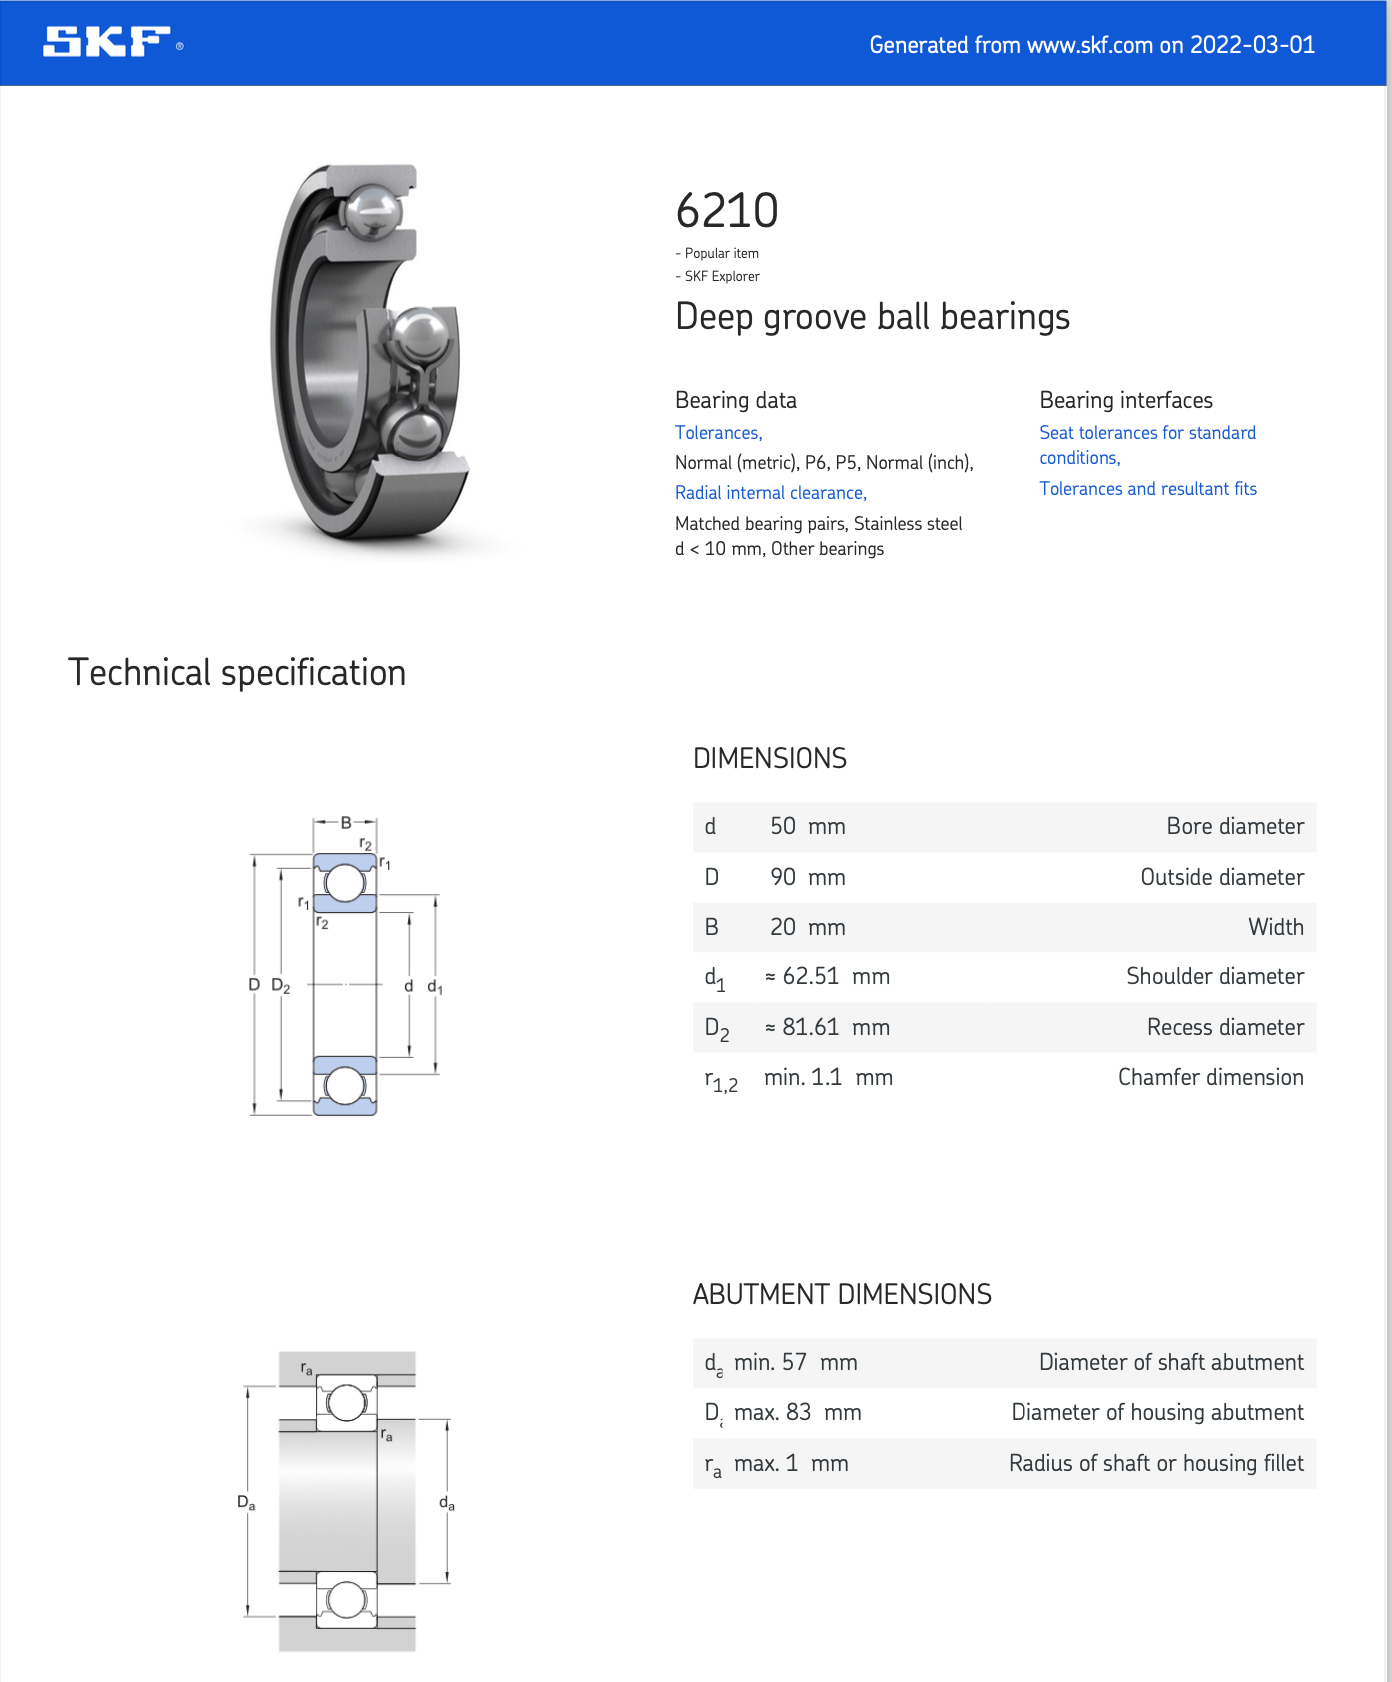
\includegraphics[scale=0.5]{Immagini/Cuscinetti1Albero1.png}
    \caption{Caratteristiche tecniche dei cuscinetti montati sull'albero 1}
    \label{fig:Cuscinetto1Albero1}
\end{figure}
\begin{figure}[h]
    \centering
    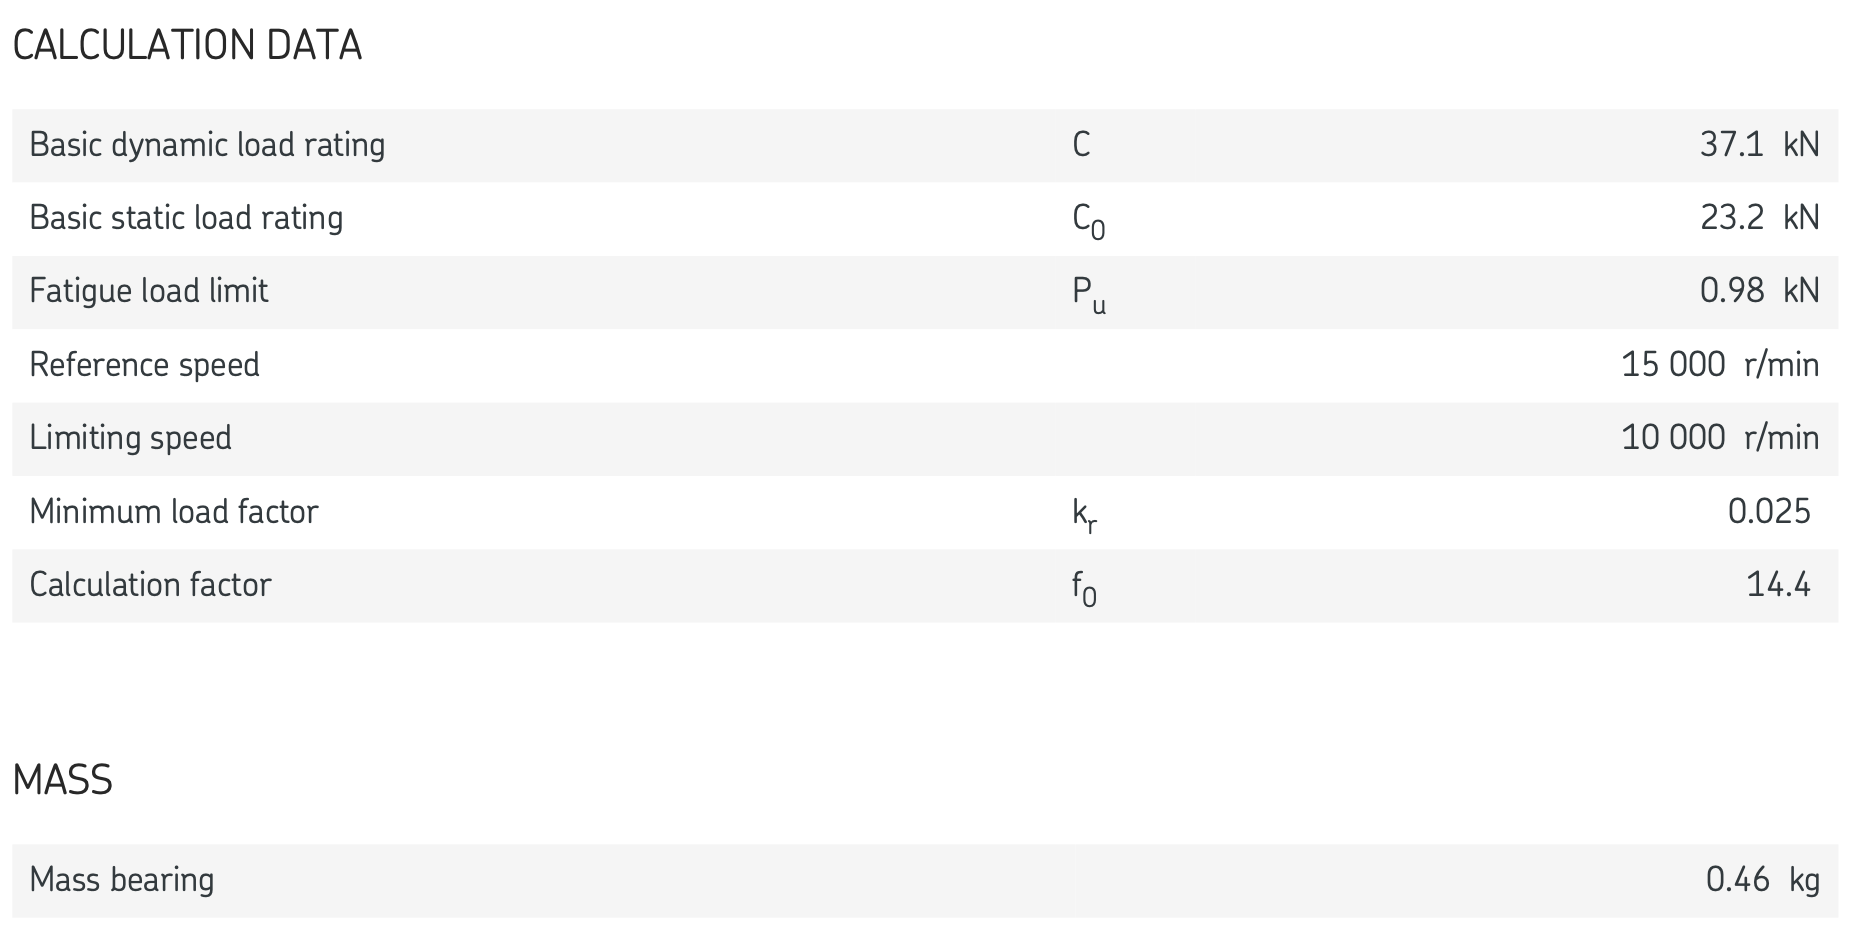
\includegraphics[scale=0.5]{Immagini/Cuscinetti2Albero1.png}
    \caption{Altre caratteristiche tecniche dei cuscinetti montati sull'albero 1}
    \label{fig:Cuscineti2Albero1}
\end{figure}

Dalla progettazione degli alberi con il software KissSoft sono stati ottenuti i seguenti risultati per i cuscinetti.
\begin{figure}[h]
    \centering
    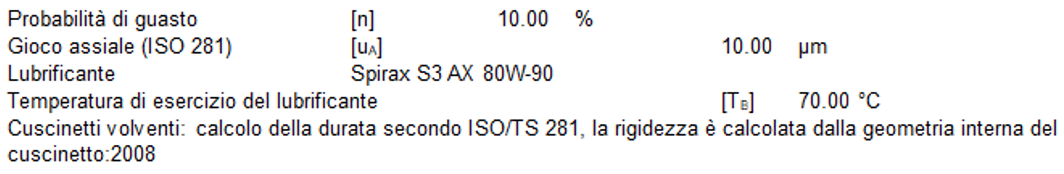
\includegraphics[scale=0.5]{Immagini/DettagliCuscinettiAlbero1.png}
    \caption{Alcuni dati notevoli riguardanti i cuscinetti dell'albero 1}
    \label{fig:DettagliCuscinettiAlbero1}
\end{figure}

Cuscinetto a sfere di sinistra.
\begin{figure}[h]
    \centering
    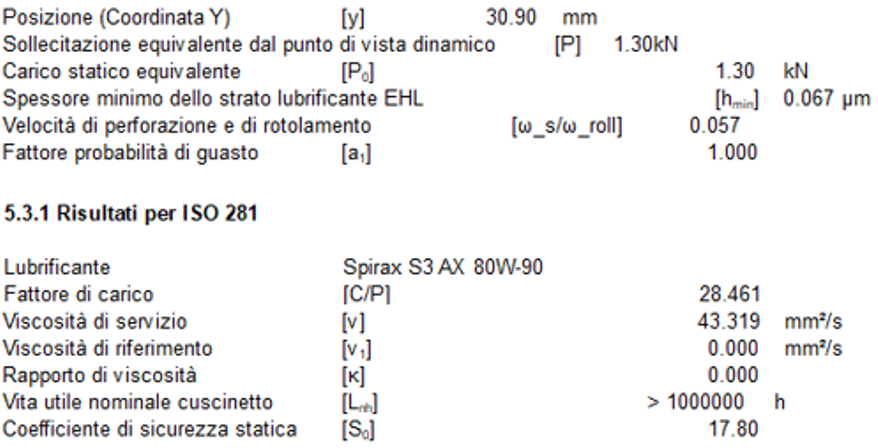
\includegraphics[scale=0.6]{Immagini/RisultatiCuscinettoSinistraAlbero1.png}
    \caption{Risultati del cuscinetto a sinistra dell'albero 1}
    \label{fig:RisultatiCuscinettoSinistraAlbero1}
\end{figure}
\newpage
Cuscinetto a sfere di destra.
\begin{figure}[h]
    \centering
    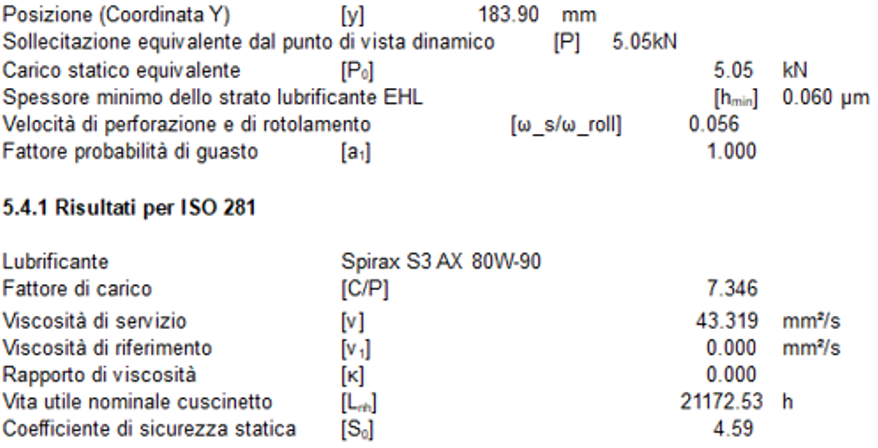
\includegraphics[scale=0.6]{Immagini/RisultatiCuscinettoDestraAlbero1.png}
    \caption{Risultati del cuscinetto di destra dell'albero 1}
    \label{fig:RisultatiCuscinettoDestraAlbero1}
\end{figure}

In conclusione.
\begin{figure}[h]
    \centering
    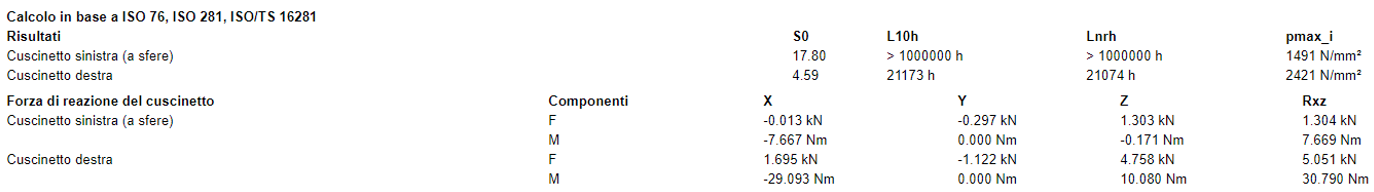
\includegraphics[scale=0.55]{Immagini/RisultatiCuscinettiAlbero1.png}
    \caption{Risultati complessivi dei cuscinetti per quanto riguarda l'albero 1}
    \label{fig:RisultatiCuscinettiAlbero1}
\end{figure}

\paragraph{Cuscinetti albero 2}
Per il secondo albero vengono utilizzati:
\begin{itemize}
    \item Cuscinetto radiale a rulli NUP 208 ECJ (lato ruota 1);
    \item Cuscinetto a rulli conici contrapposti ad “o” 30212T53/DB (lato ruota 2)
\end{itemize}
\newpage
\begin{figure}[h]
    \centering
    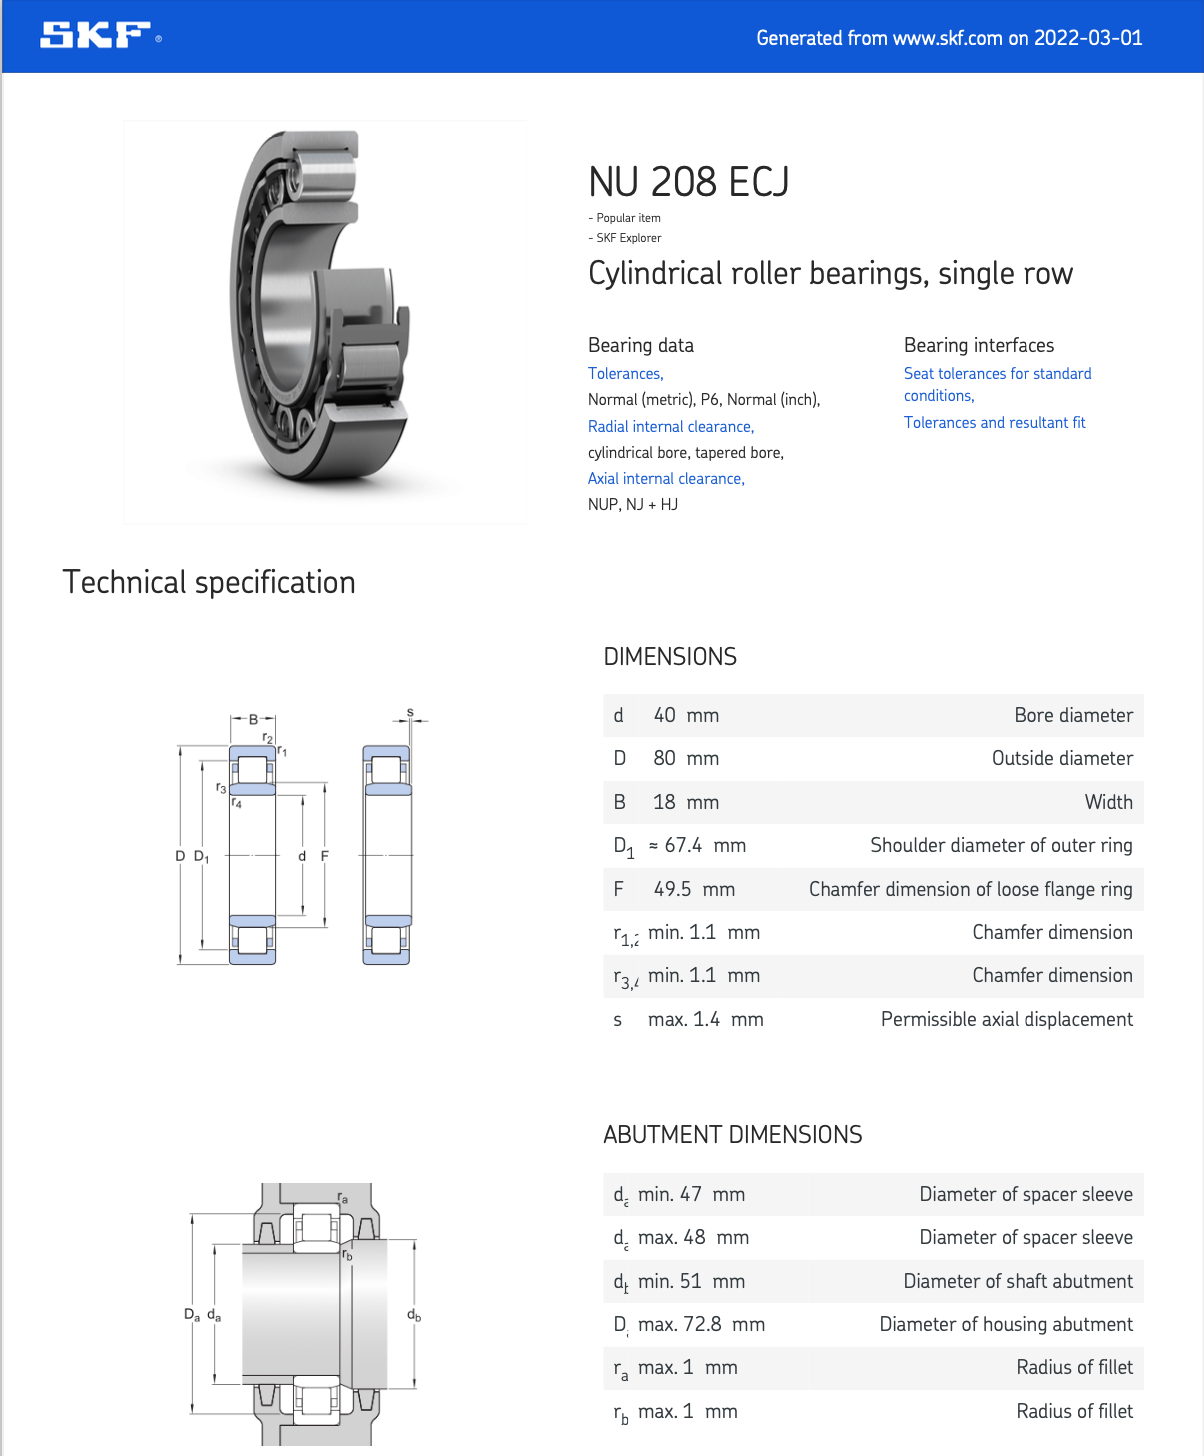
\includegraphics[scale=0.6]{Immagini/Cuscinetti1Albero2.png}
    \caption{Caratteristiche tecniche dei cuscinetti montati sull'albero 2}
    \label{fig:Cuscinetti1Albero1}
\end{figure}
\newpage
\begin{figure}[h]
    \centering
    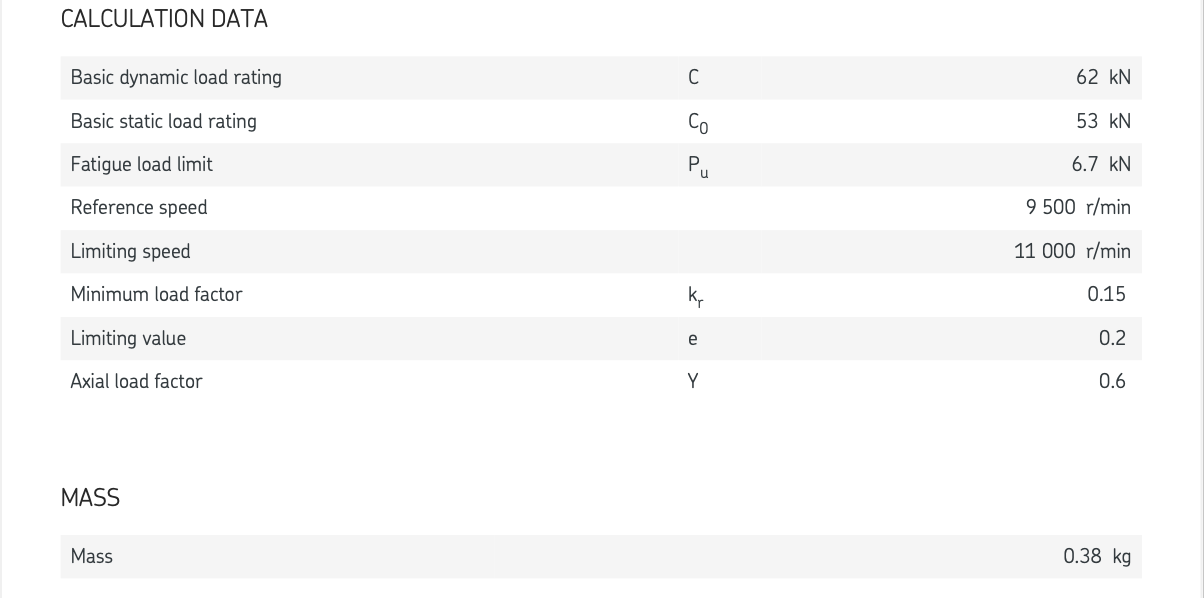
\includegraphics[scale=0.6]{Immagini/Cuscinetti2Albero2.png}
    \caption{Altre caratteristiche tecniche dei cuscinetti montati sull'albero 1}
    \label{fig:Cuscinetti2Albero1}
\end{figure}
\newpage
\begin{figure}[h]
    \centering
    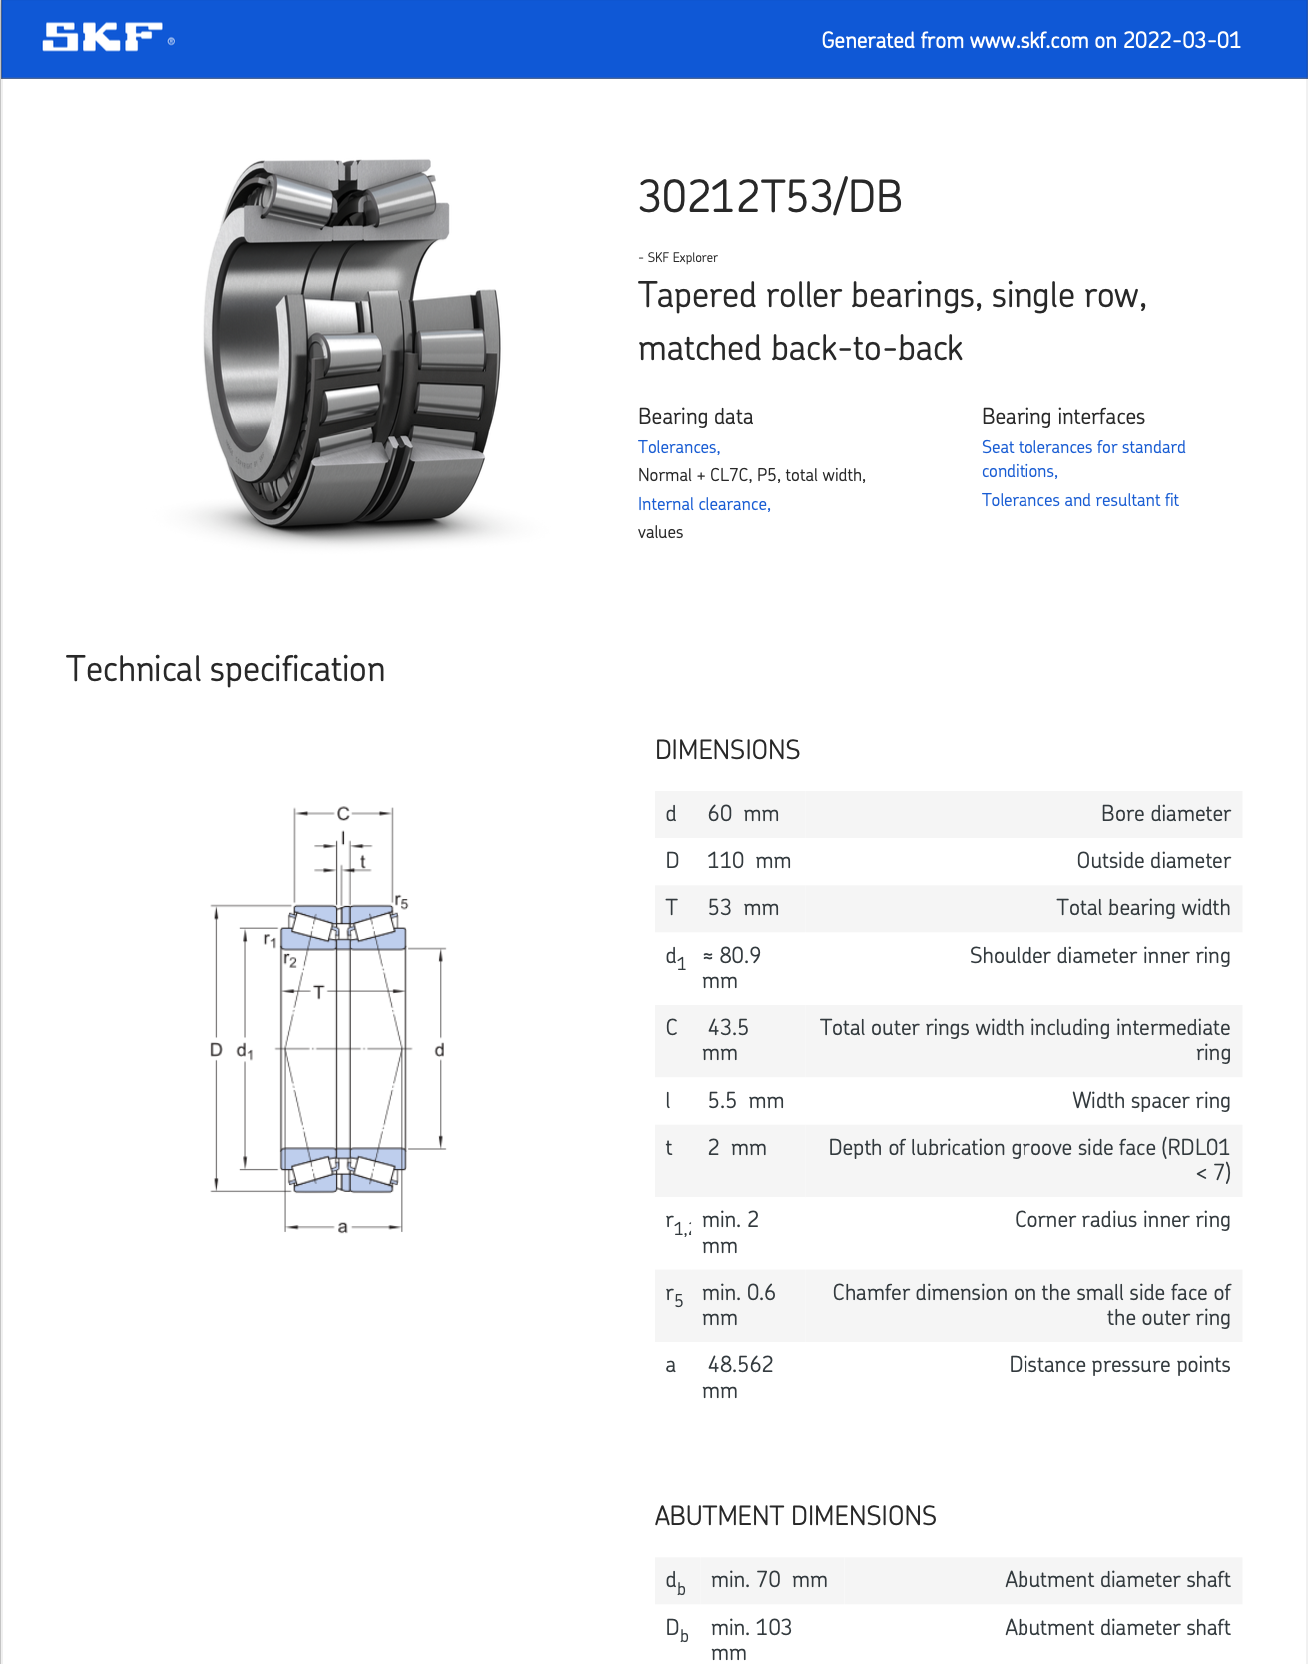
\includegraphics[scale=0.6]{Immagini/Cuscinetti3Albero2.png}
    \caption{Caratteristiche tecniche dei cuscinetti montati sull'albero 2}
    \label{fig:Cuscinetti3Albero2}
\end{figure}
\newpage
\begin{figure}[h]
    \centering
    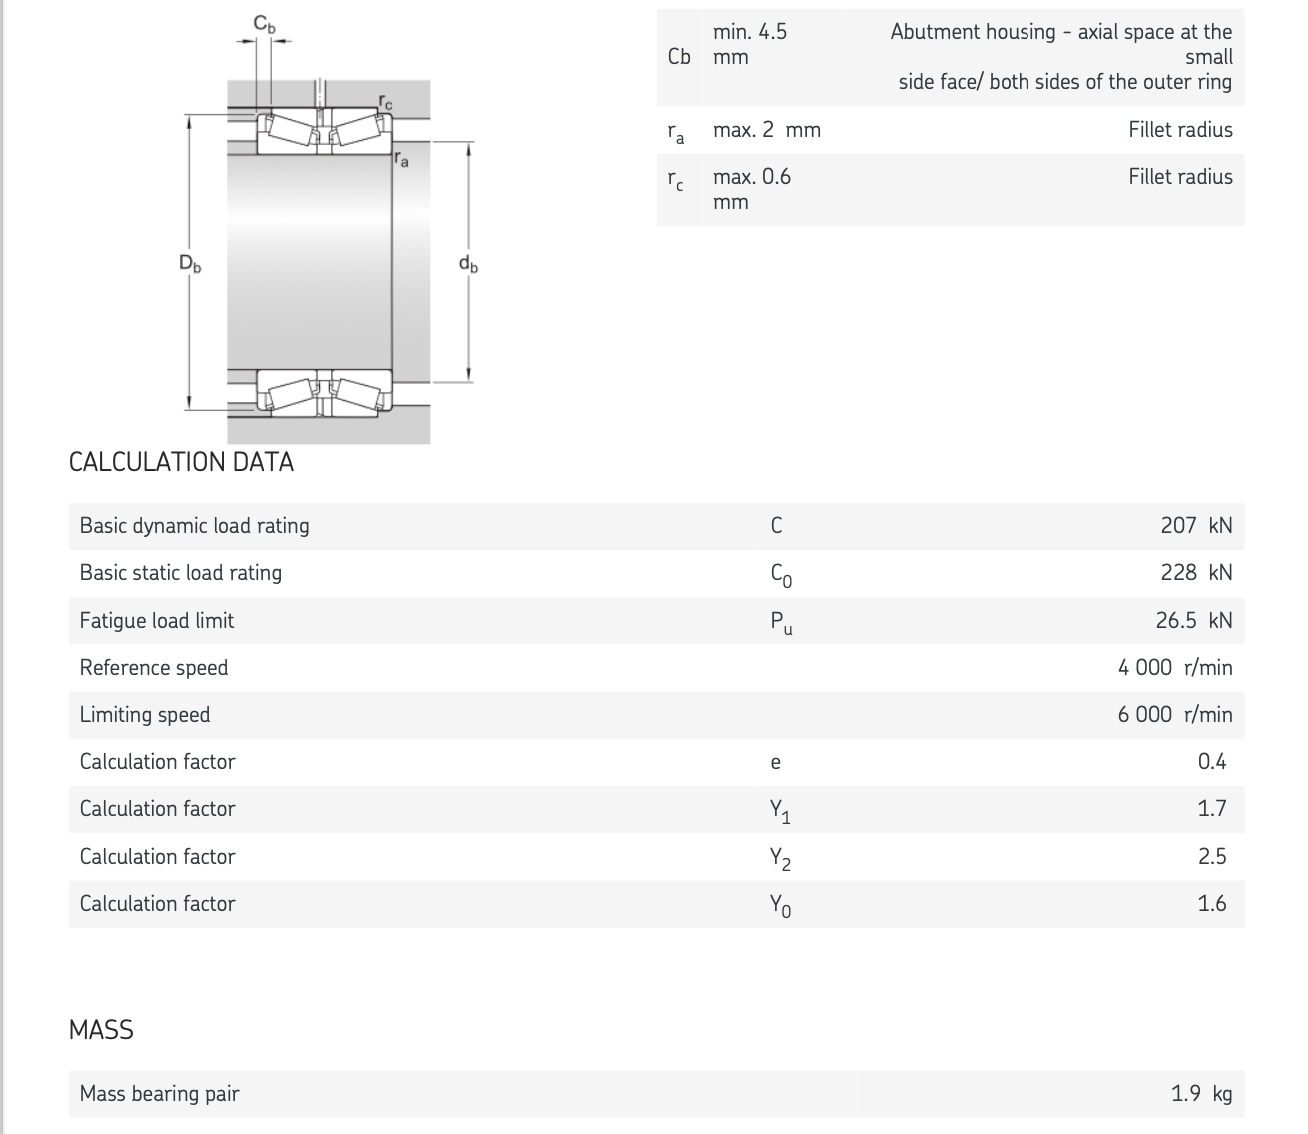
\includegraphics[scale=0.6]{Immagini/Cuscinetti4Albero2.png}
    \caption{Altre caratteristiche tecniche dei cuscinetti montati sull'albero 2}
    \label{fig:Cuscinetti4Albero2}
\end{figure}

Dalla progettazione degli alberi con il software KissSoft sono stati ottenuti i seguenti risultati per i cuscinetti.
\begin{figure}[h]
    \centering
    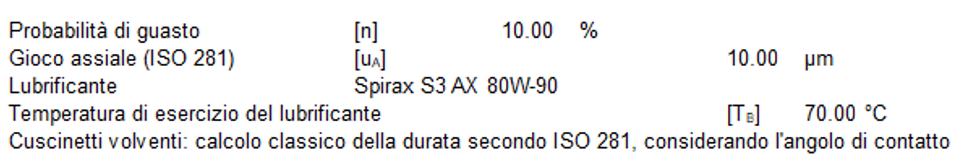
\includegraphics[scale=0.6]{Immagini/DettagliCuscinettiAlbero2.png}
    \caption{Alcuni dati notevoli riguardanti i cuscinetti dell'albero 2}
    \label{fig:DettagliCuscinettiAlbero2}
\end{figure}
\newpage
Cuscinetto a rulli di sinistra.
\begin{figure}[h]
    \centering
        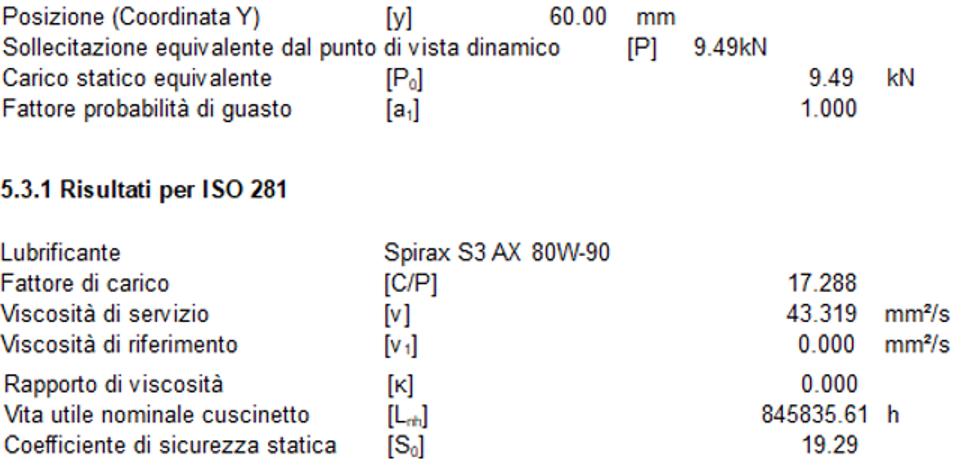
\includegraphics[scale=0.6]{Immagini/RisultatiCuscinettoSinistraAlbero2.png}
    \caption{Risultati del cuscinetto a sinistra dell'albero 2}
    \label{fig:RisultatiCuscinettoSinistraAlbero2}
\end{figure}

Cuscinetto a rulli di destra.
\begin{figure}[h]
    \centering
    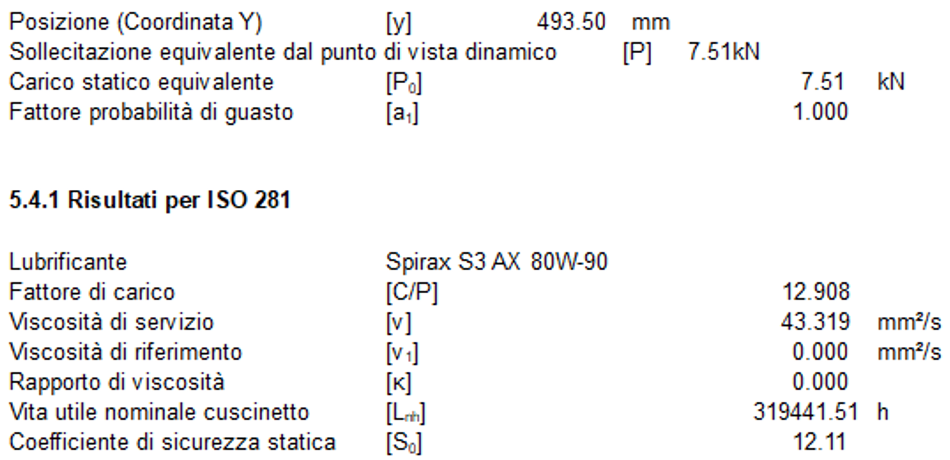
\includegraphics[scale=0.6]{Immagini/RisultatiCuscinettoDestraAlbero2.png}
    \caption{Risultati del cuscinetto di destra dell'albero 2}
    \label{fig:RisultatiCuscinettoDestraAlbero2}
\end{figure}

In conclusione.
\begin{figure}[h]
    \centering
    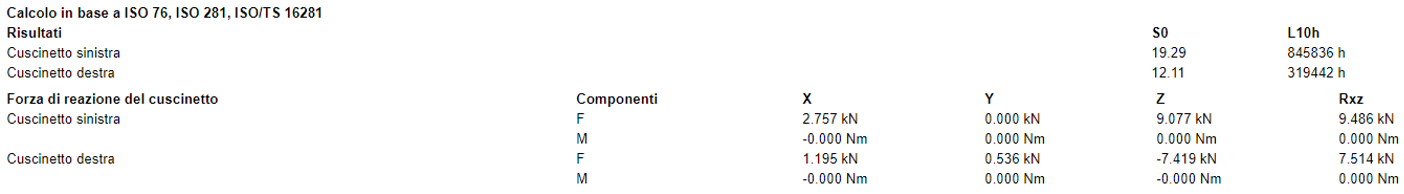
\includegraphics[scale=0.55]{Immagini/RisultatiCuscinettiAlbero2.png}
    \caption{Risultati complessivi dei cuscinetti per quanto riguarda l'albero 2}
    \label{fig:RisultatiCuscinettiAlbero2}
\end{figure}

\paragraph{Cuscinetti albero 3 }
Per il terzo albero sono stati utilizzati 2 cuscinetti radiali a rulli conici 30207. 
\newpage
\begin{figure}[h]
    \centering
    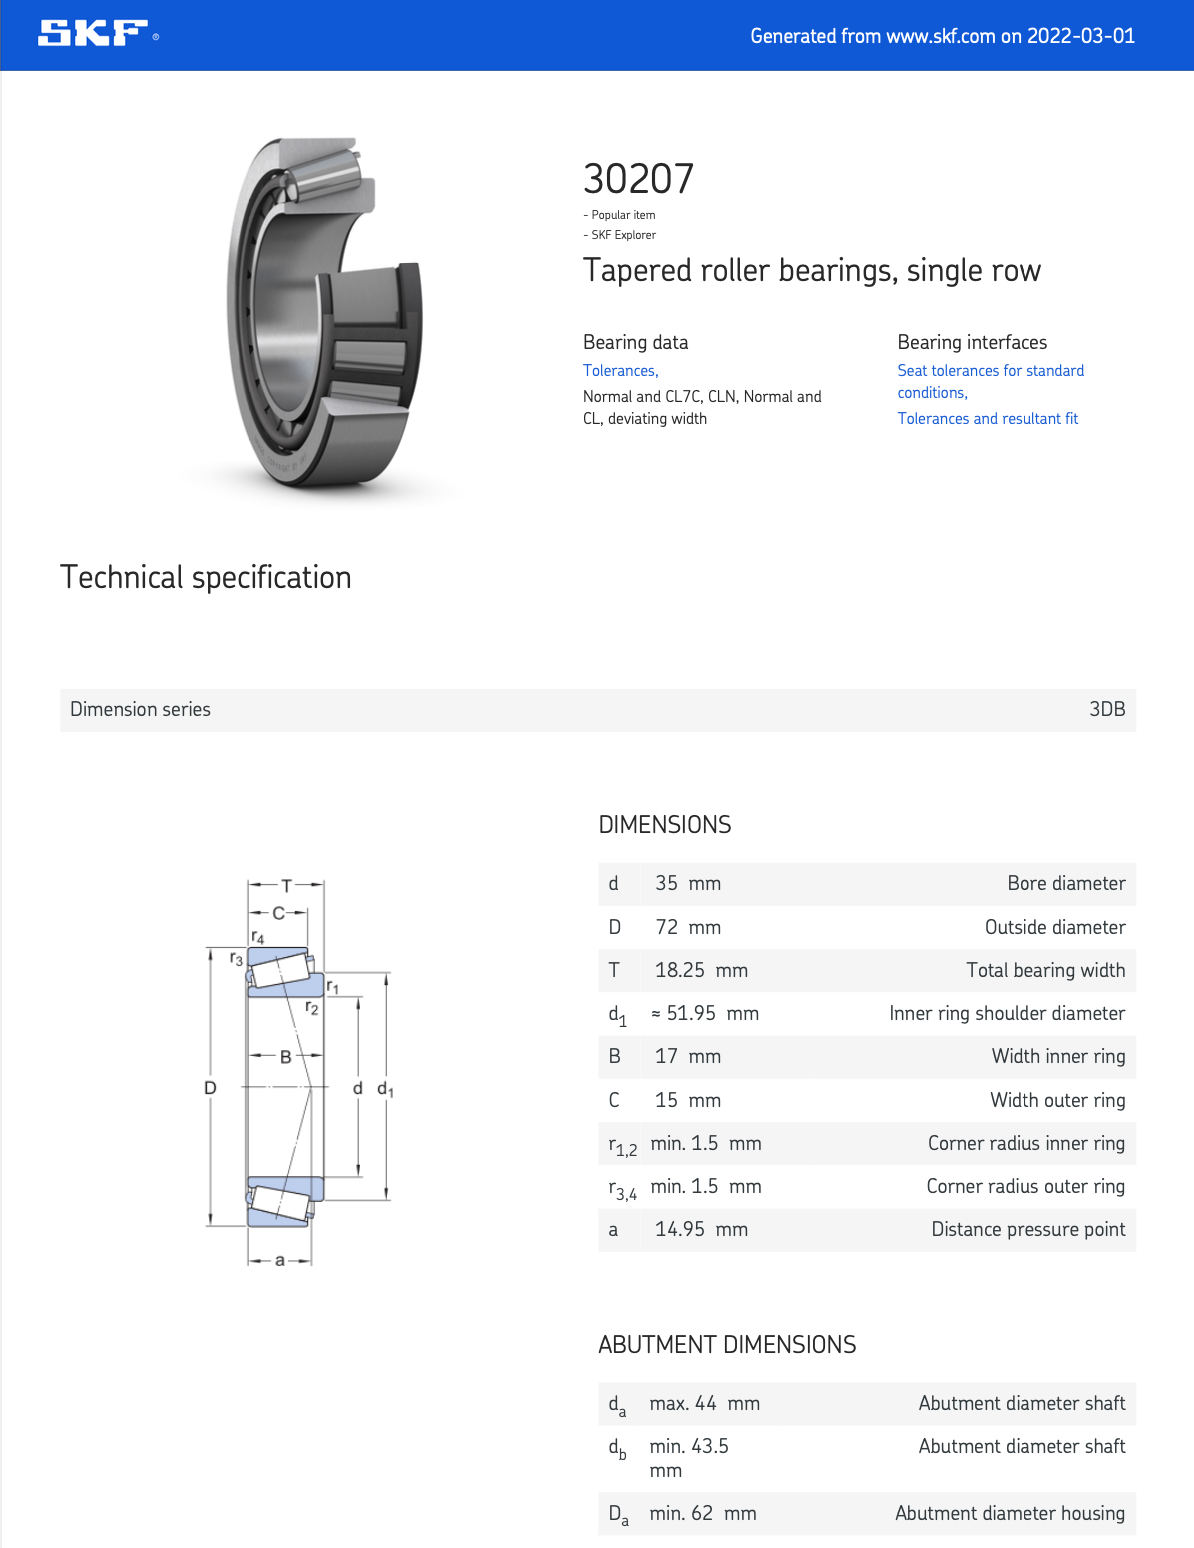
\includegraphics[scale=0.6]{Immagini/Cuscinetti1Albero3.png}
    \caption{Caratteristiche tecniche dei cuscinetti montati sull'albero 3}
    \label{fig:Cuscinetto1Albero3}
\end{figure}
\newpage
\begin{figure}[h]
    \centering
    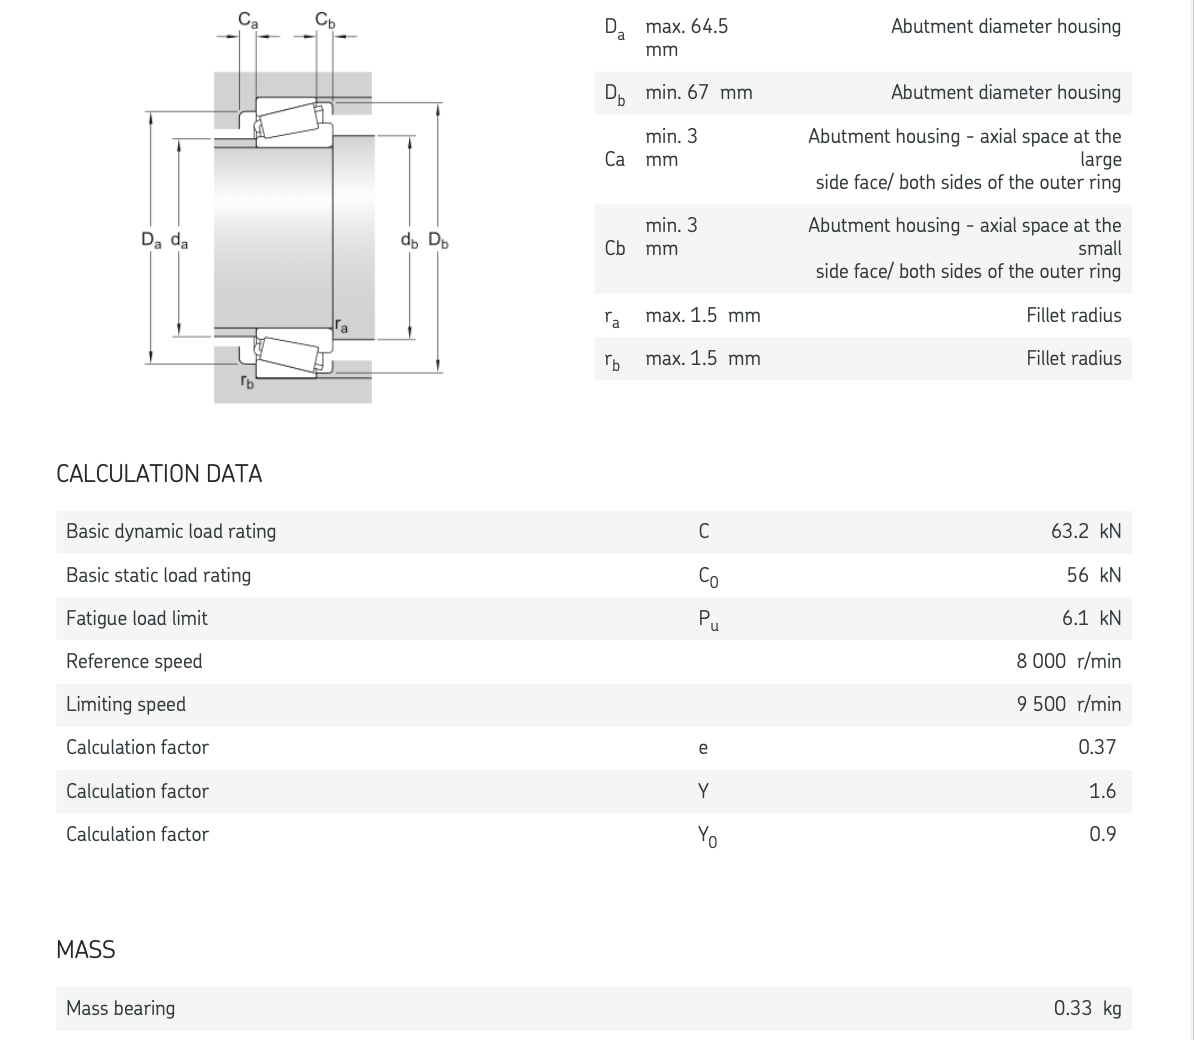
\includegraphics[scale=0.6]{Immagini/Cuscinetti2Albero3.png}
    \caption{Altre caratteristiche tecniche dei cuscinetti montati sull'albero 3}
    \label{fig:Cuscineti2Albero3}
\end{figure}

Dalla progettazione degli alberi con il software KissSoft sono stati ottenuti i seguenti risultati per i cuscinetti.
\begin{figure}[h]
    \centering
    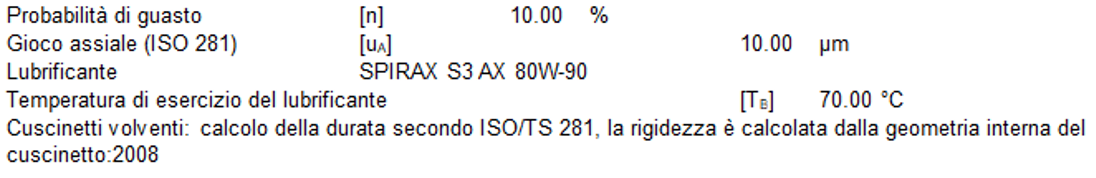
\includegraphics[scale=0.6]{Immagini/DettagliCuscinettiAlbero3.png}
    \caption{Alcuni dati notevoli riguardanti i cuscinetti dell'albero 3}
    \label{fig:DettagliCuscinettiAlbero3}
\end{figure}
\newpage
\emph{Step 1}\\
Cuscinetto a rulli in basso.
\begin{figure}[h]
    \centering
    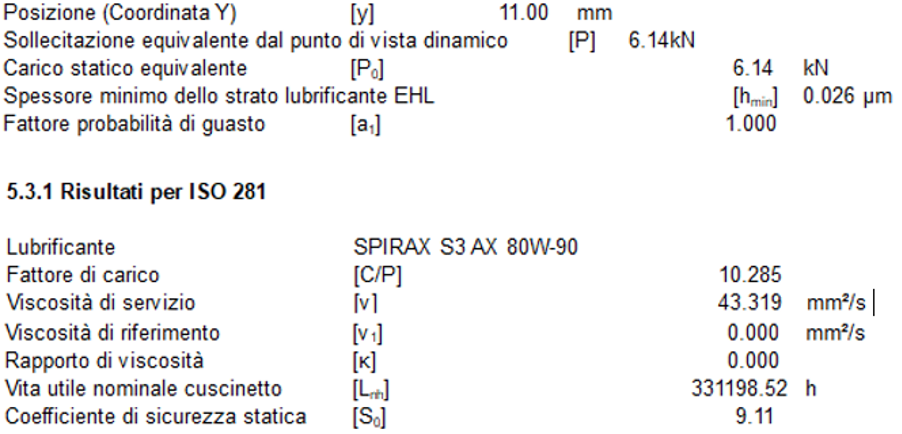
\includegraphics[scale=0.6]{Immagini/RisultatiCuscinettoBasso1Albero3.png}
    \caption{Risultati del cuscinetto in basso dell'albero 3}
    \label{fig:RisultatiCuscinettoBasso1Albero3}
\end{figure}

Cuscinetto a rulli in alto.
\begin{figure}[h]
    \centering
    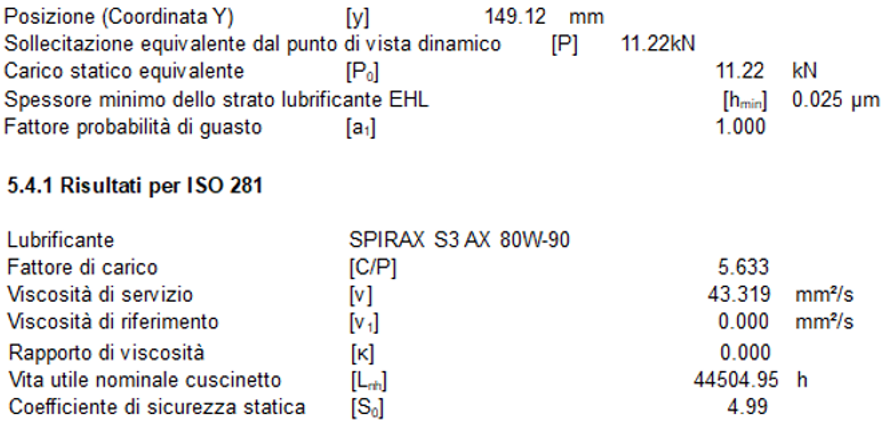
\includegraphics[scale=0.6]{Immagini/RisultatiCuscinettoAlto1Albero3.png}
    \caption{Risultati del cuscinetto in alto dell'albero 3}
    \label{fig:RisultatiCuscinettoAlto1Albero3}
\end{figure}

In conclusione.
\begin{figure}[h]
    \centering
    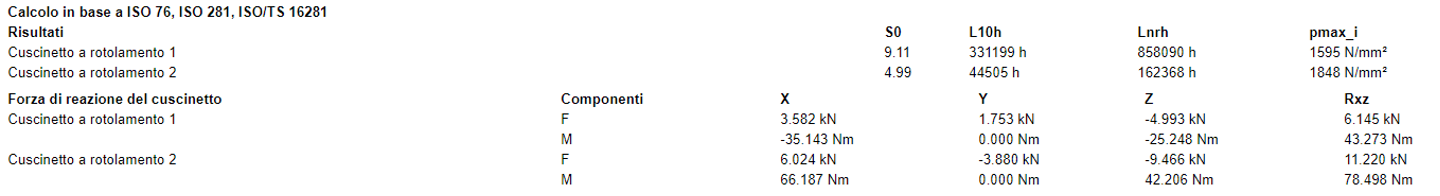
\includegraphics[scale=0.55]{Immagini/RisultatiCuscinetti1Albero3.png}
    \caption{Risultati complessivi dei cuscinetti nello step 1 per quanto riguarda l'albero 3}
    \label{fig:RisultatiCuscinetti1Albero3}
\end{figure}
\newpage
\emph{Step 2}\\
Cuscinetto a rulli in basso.
\begin{figure}[h]
    \centering
    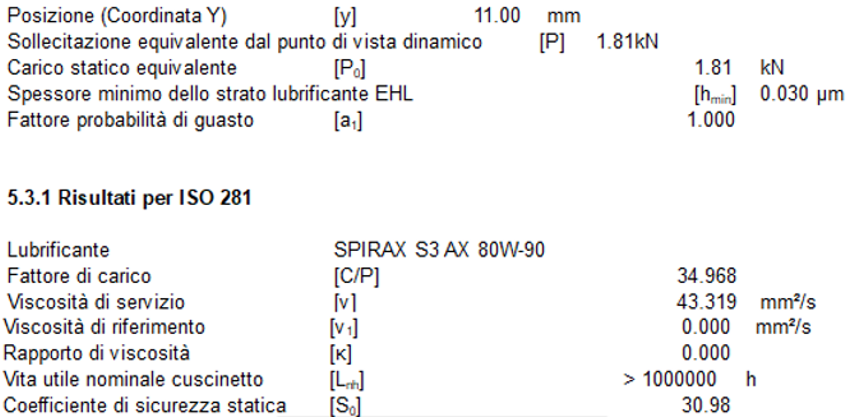
\includegraphics[scale=0.6]{Immagini/RisultatiCuscinettoBasso2Albero3.png}
    \caption{Risultati del cuscinetto in basso dell'albero 3}
    \label{fig:RisultatiCuscinettoBasso2Albero3}
\end{figure}

Cuscinetto a rulli in alto.
\begin{figure}[h]
    \centering
    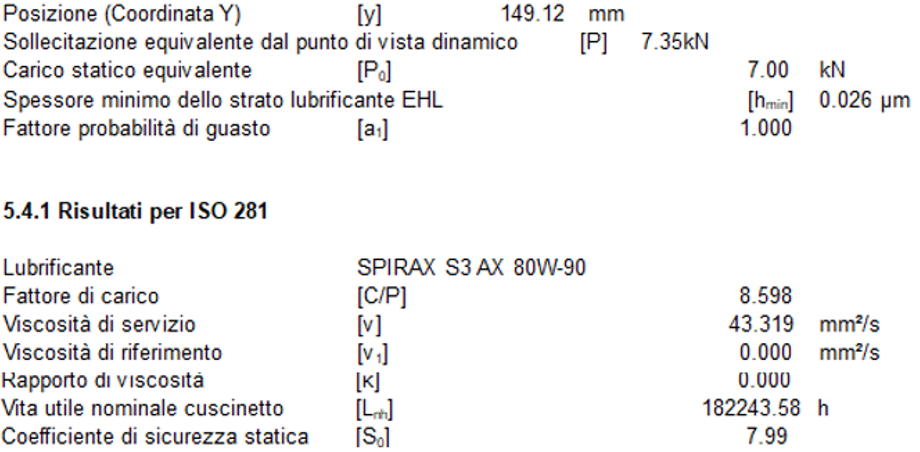
\includegraphics[scale=0.6]{Immagini/RisultatiCuscinettoAlto2Albero3.png}
    \caption{Risultati del cuscinetto in alto dell'albero 3}
    \label{fig:RisultatiCuscinettoAlto2Albero3}
\end{figure}

In conclusione.
\begin{figure}[h]
    \centering
    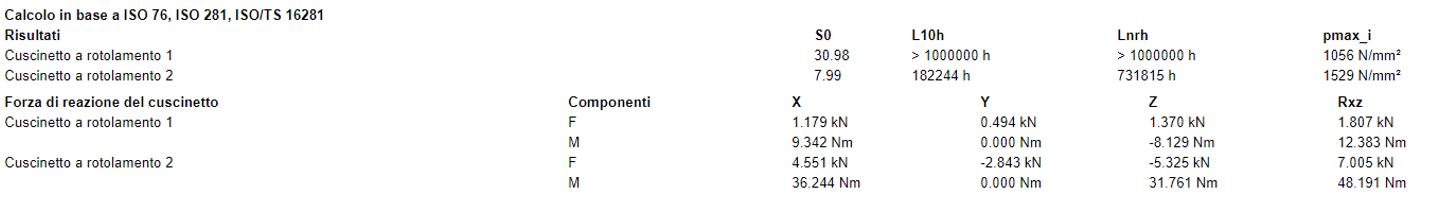
\includegraphics[scale=0.55]{Immagini/RisultatiCuscinetti2Albero3.png}
    \caption{Risultati complessivi dei cuscinetti nello step 2 per quanto riguarda l'albero 3}
    \label{fig:RisultatiCuscinetti2Albero3}
\end{figure}
\newpage
\emph{Step 3}\\
Cuscinetto a rulli in basso.
\begin{figure}[h]
    \centering
    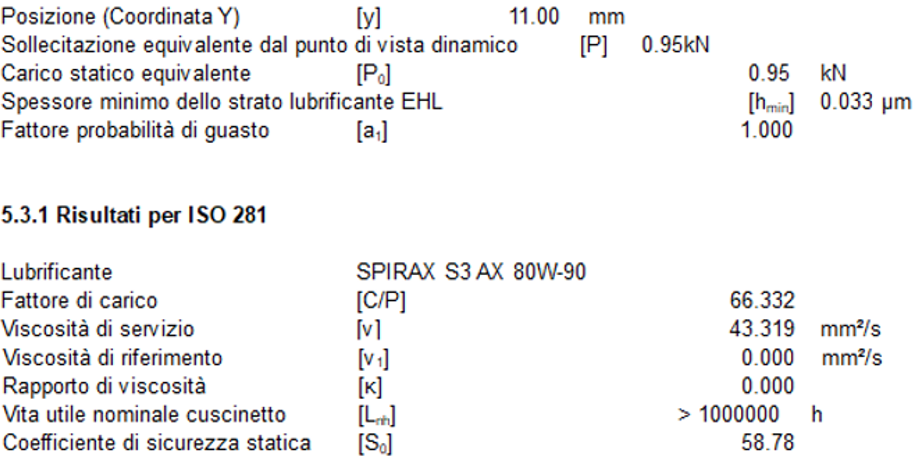
\includegraphics[scale=0.6]{Immagini/RisultatiCuscinettoBasso3Albero3.png}
    \caption{Risultati del cuscinetto in basso dell'albero 3}
    \label{fig:RisultatiCuscinettoBassoAlbero3}
\end{figure}

Cuscinetto a rulli in alto.
\begin{figure}[h]
    \centering
    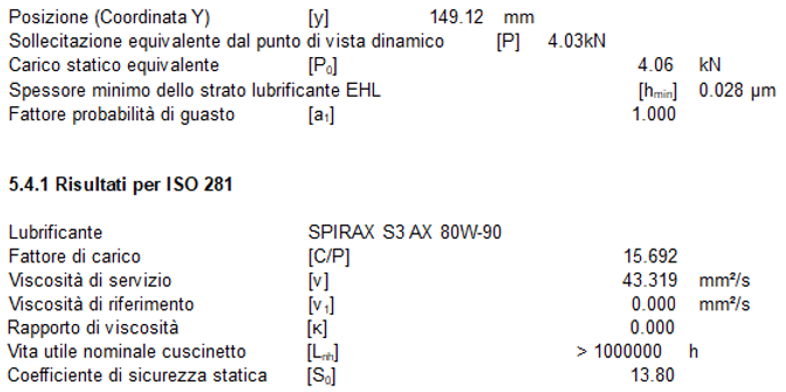
\includegraphics[scale=0.6]{Immagini/RisultatiCuscinettoAlto3Albero3.png}
    \caption{Risultati del cuscinetto in alto dell'albero 3}
    \label{fig:RisultatiCuscinettoAlto3Albero3}
\end{figure}

In conclusione.
\begin{figure}[h]
    \centering
    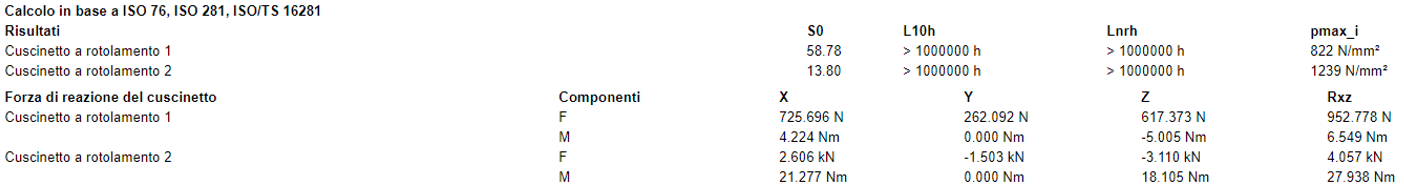
\includegraphics[scale=0.55]{Immagini/RisultatiCuscinetti3Albero3.png}
    \caption{Risultati complessivi dei cuscinetti nello step 3 per quanto riguarda l'albero 3}
    \label{fig:RisultatiCuscinetti3Albero3}
\end{figure}

In conclusione, in tutte e tre le configurazioni i cuscinetti soddisfano la vita utile richiesta. 
\paragraph{Albero 4 (output 1)}
Per il quarto albero vengono utilizzati:
\begin{itemize}
    \item Cuscinetto radiale a rulli NUP 211 ECJ (parte inferiore dell’albero);
    \item Cuscinetto radiale a sfere 6210 (nella parte superiore dell’albero), le cui caratteristiche sono state precedentemente definite nell’albero 1 di input. 
\end{itemize}
\newpage
\begin{figure}[h]
    \centering
    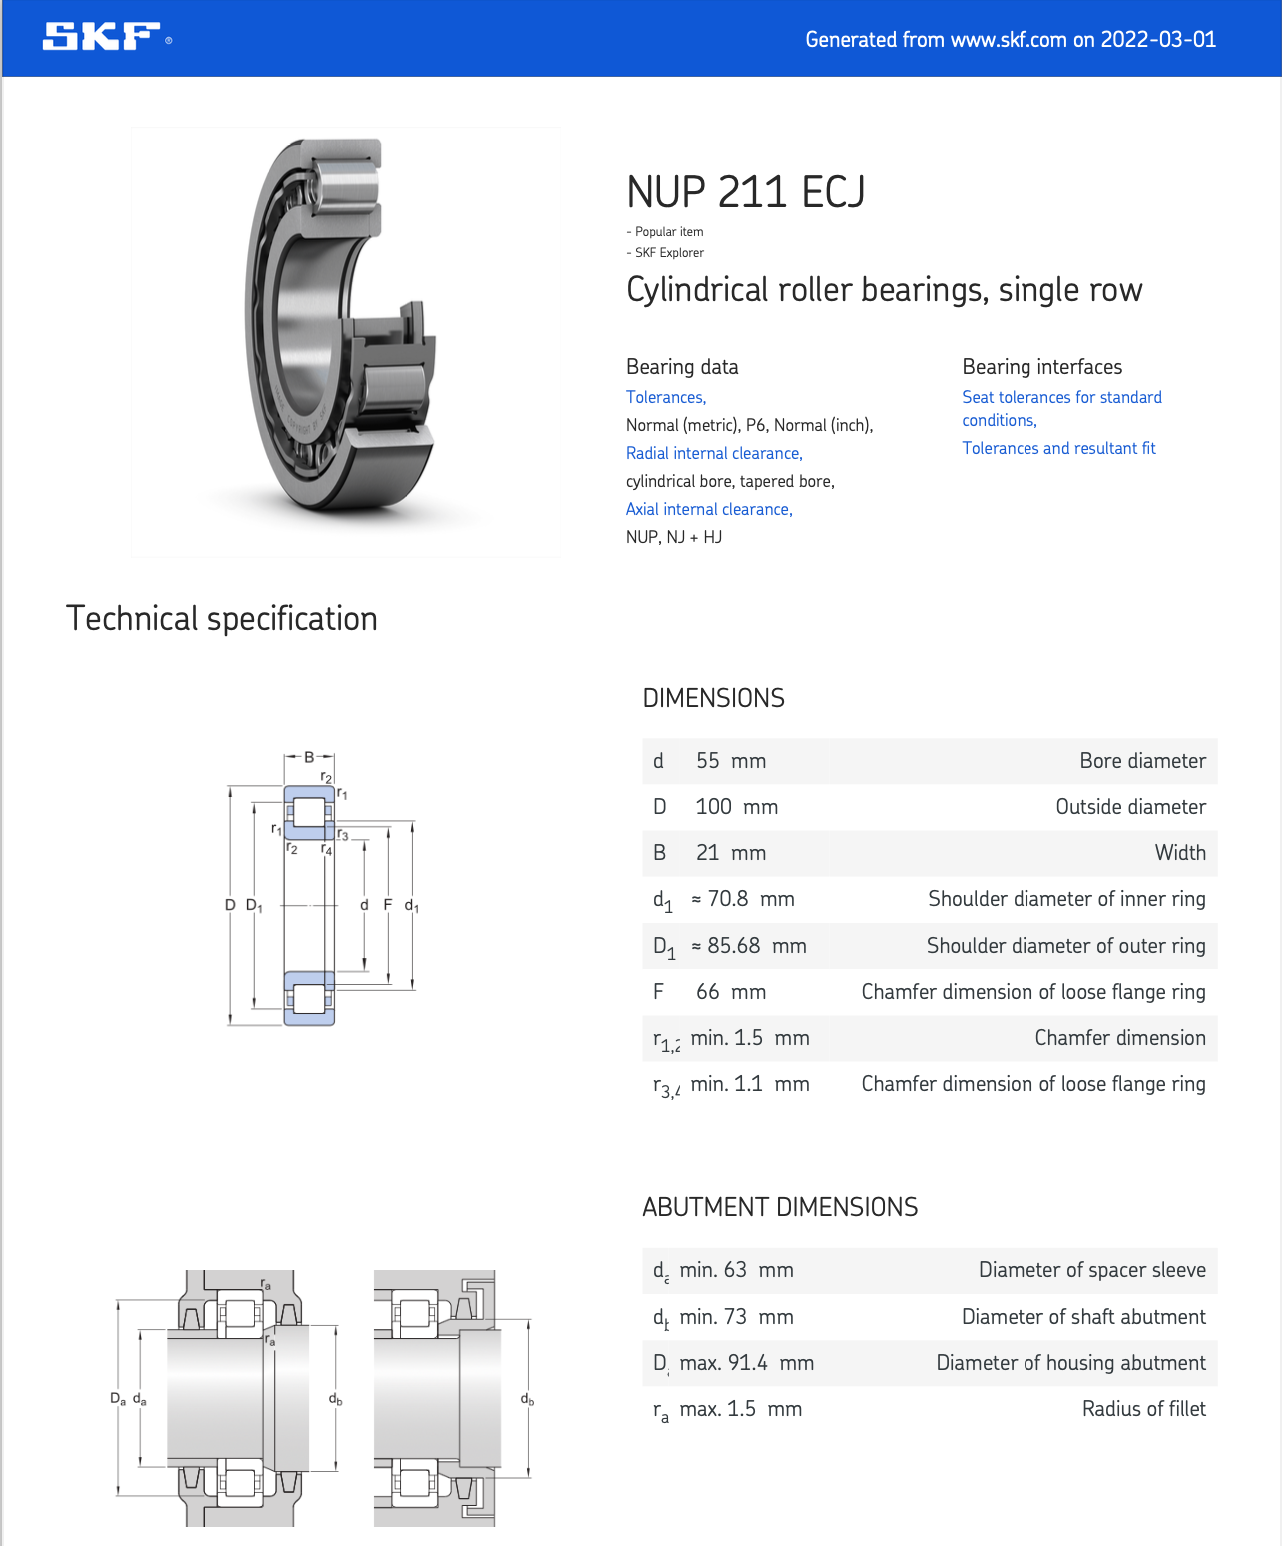
\includegraphics[scale=0.6]{Immagini/Cuscinetti1Albero4.png}
    \caption{Caratteristiche tecniche dei cuscinetti montati sull'albero 4}
    \label{fig:Cuscinetti1Albero4}
\end{figure}
\newpage
\begin{figure}[h]
    \centering
    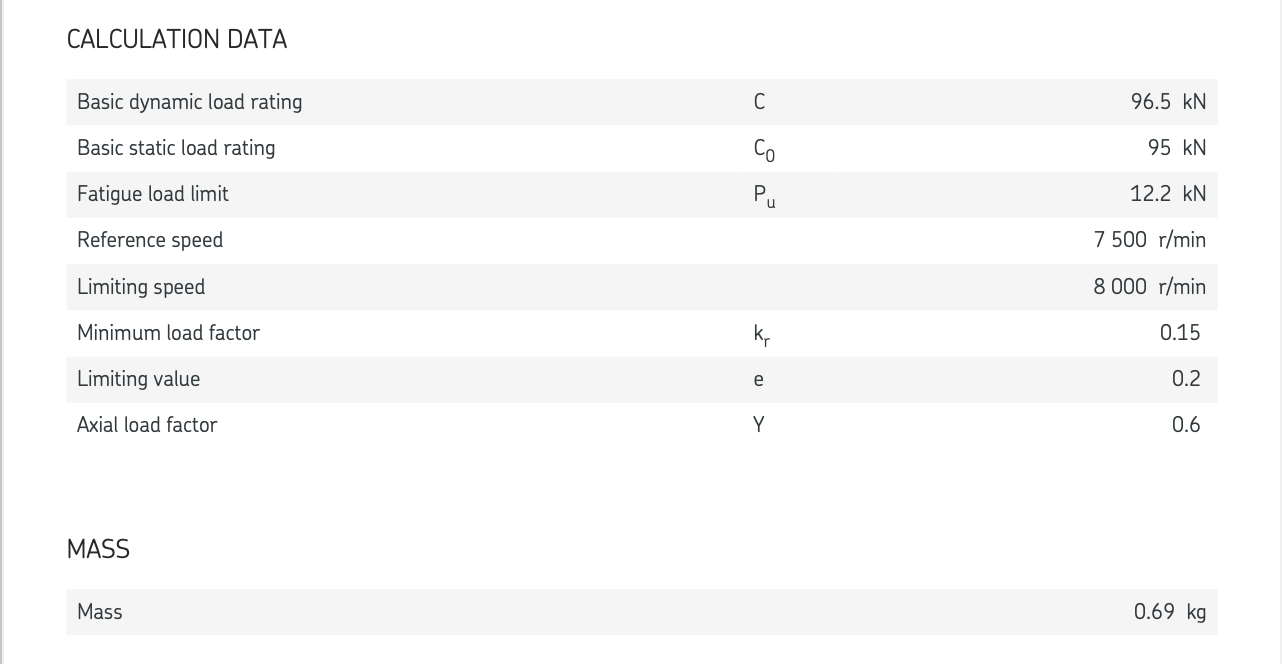
\includegraphics[scale=0.6]{Immagini/Cuscinetti2Albero4.png}
    \caption{Altre caratteristiche tecniche dei cuscinetti montati sull'albero 4}
    \label{fig:Cuscinetti2Albero4}
\end{figure}

Dalla progettazione degli alberi con il software KissSoft sono stati ottenuti i seguenti risultati per i cuscinetti.
\begin{figure}[h]
    \centering
    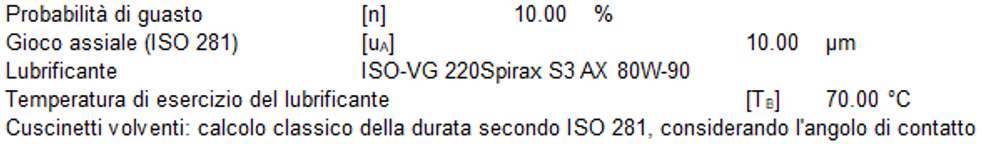
\includegraphics[scale=0.6]{Immagini/DettagliCuscinettiAlbero4.png}
    \caption{Alcuni dati notevoli riguardanti i cuscinetti dell'albero 4}
    \label{fig:DettagliCuscinettiAlbero4}
\end{figure}

Cuscinetto a rulli in basso.
\begin{figure}[h]
    \centering
        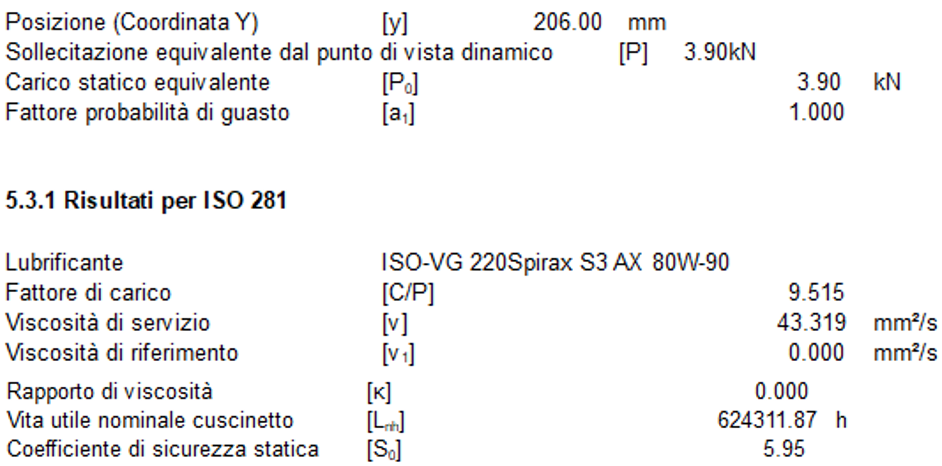
\includegraphics[scale=0.6]{Immagini/RisultatiCuscinettoBassoAlbero4.png}
    \caption{Risultati del cuscinetto in basso dell'albero 4}
    \label{fig:RisultatiCuscinettoBassoAlbero4}
\end{figure}
\newpage
Cuscinetto a sfere in alto.
\begin{figure}[h]
    \centering
    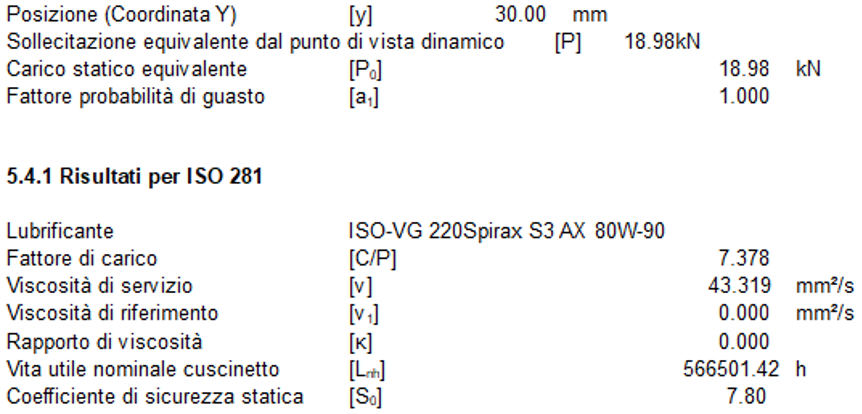
\includegraphics[scale=0.6]{Immagini/RisultatiCuscinettoAltoAlbero4.png}
    \caption{Risultati del cuscinetto in alto dell'albero 4}
    \label{fig:RisultatiCuscinettoAltoAlbero4}
\end{figure}

In conclusione.
\begin{figure}[h]
    \centering
    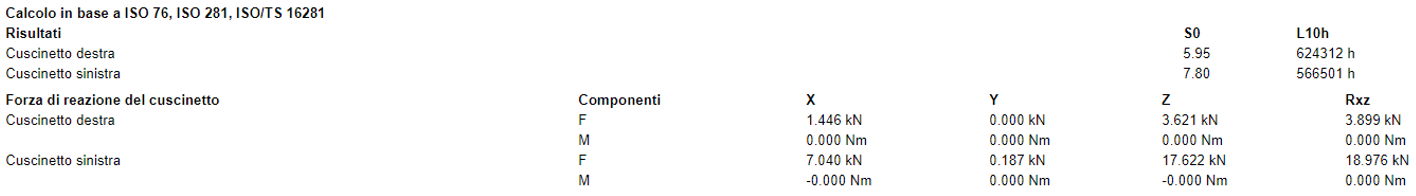
\includegraphics[scale=0.55]{Immagini/RisultatiCuscinettiAlbero4.png}
    \caption{Risultati complessivi dei cuscinetti per quanto riguarda l'albero 4}
    \label{fig:RisultatiCuscinettiAlbero4}
\end{figure}

\paragraph{Albero 5 (output 2)}
Per il quinto albero sono stati scelti:
\begin{itemize}
    \item Cuscinetto radiale a rulli NUP 212 ECJ (nella parte inferiore dell’albero);
    \item Cuscinetto radiale a sfere 61822 (nella parte superiore dell’albero).
\end{itemize}
\newpage
\begin{figure}[h]
    \centering
    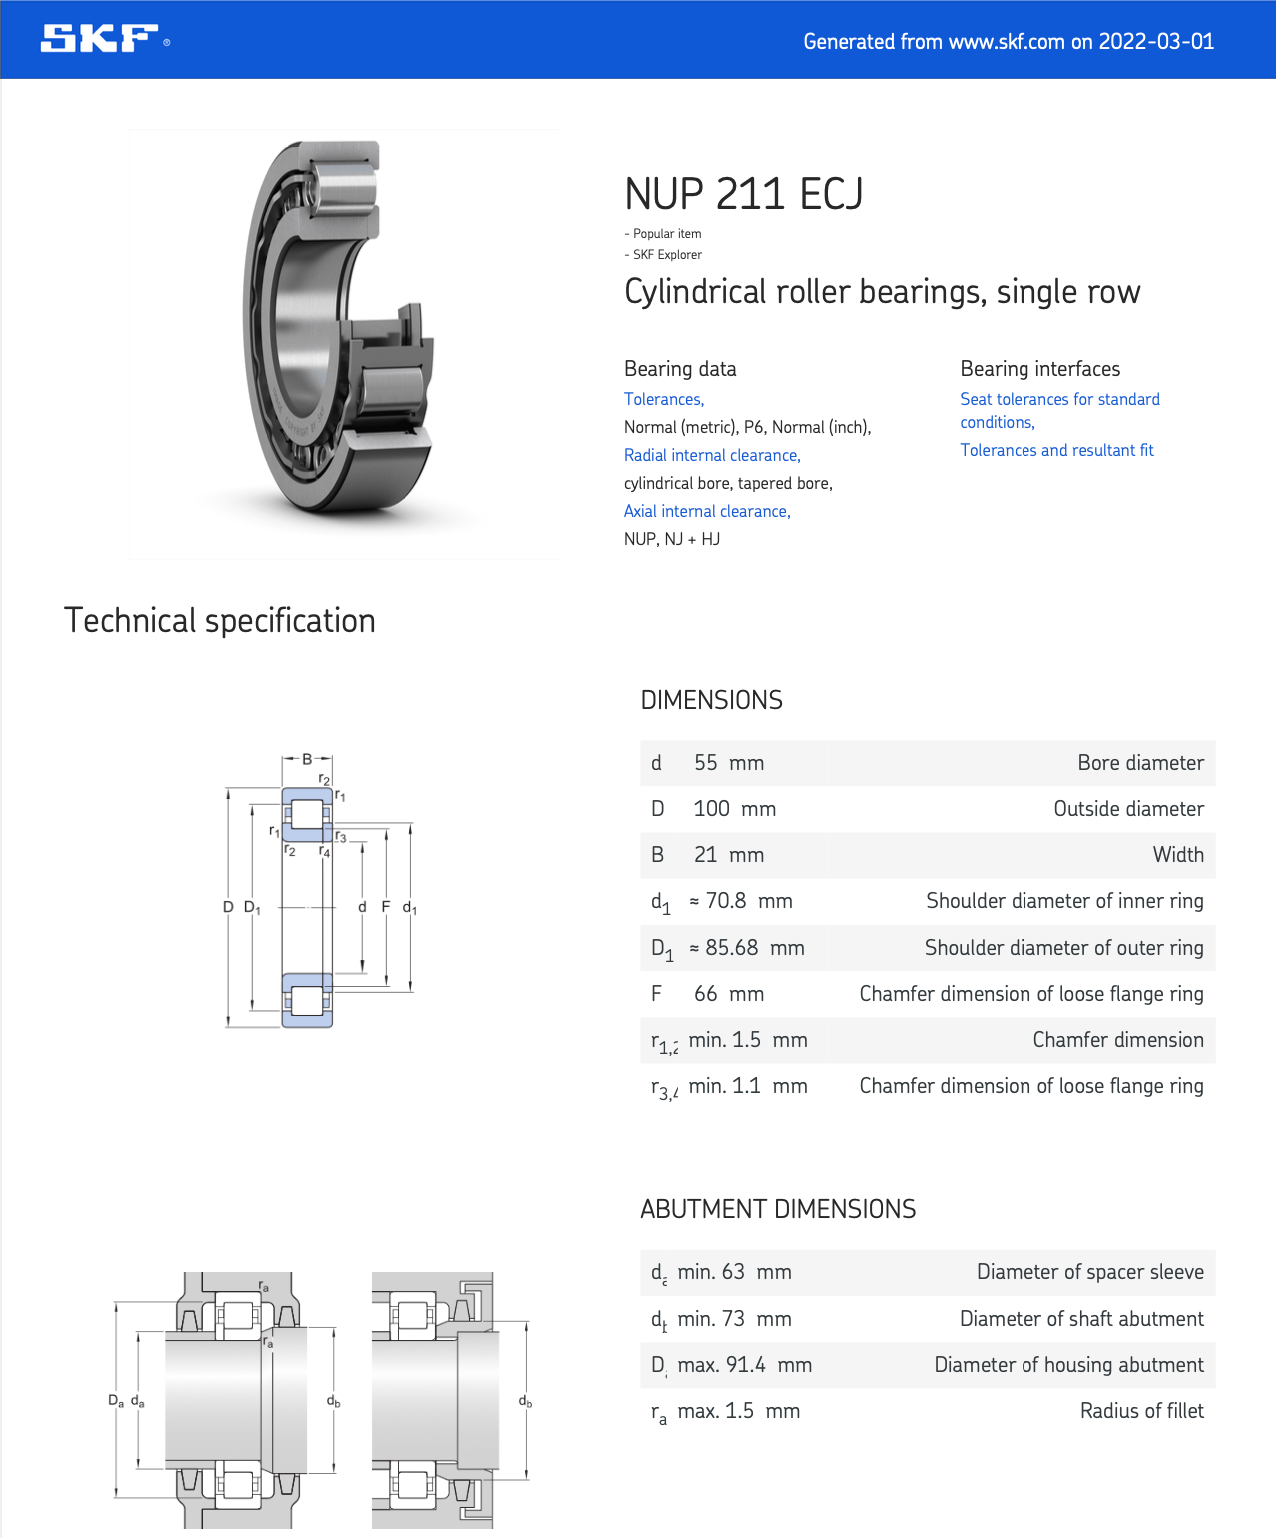
\includegraphics[scale=0.6]{Immagini/Cuscinetti1Albero5.png}
    \caption{Caratteristiche tecniche dei cuscinetti montati sull'albero 5}
    \label{fig:Cuscinetti1Albero5}
\end{figure}
\newpage
\begin{figure}[h]
    \centering
    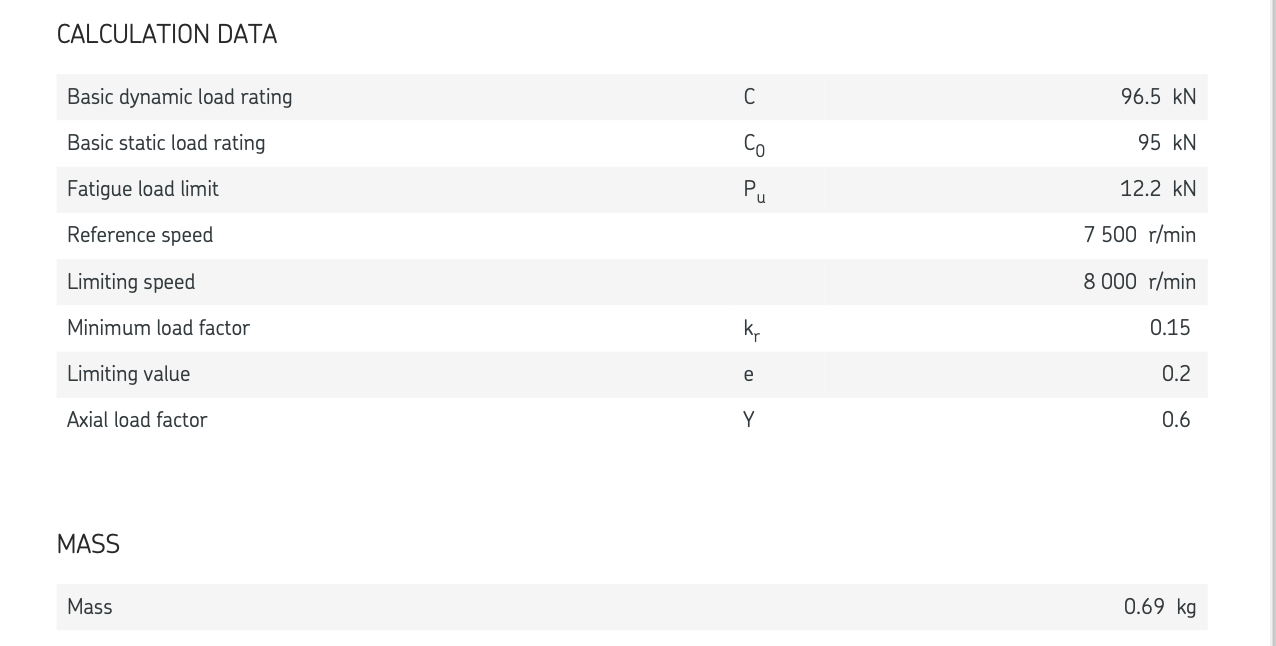
\includegraphics[scale=0.6]{Immagini/Cuscinetti2Albero5.png}
    \caption{Altre caratteristiche tecniche dei cuscinetti montati sull'albero 5}
    \label{fig:Cuscinetti2Albero5}
\end{figure}
\newpage
\begin{figure}[h]
    \centering
    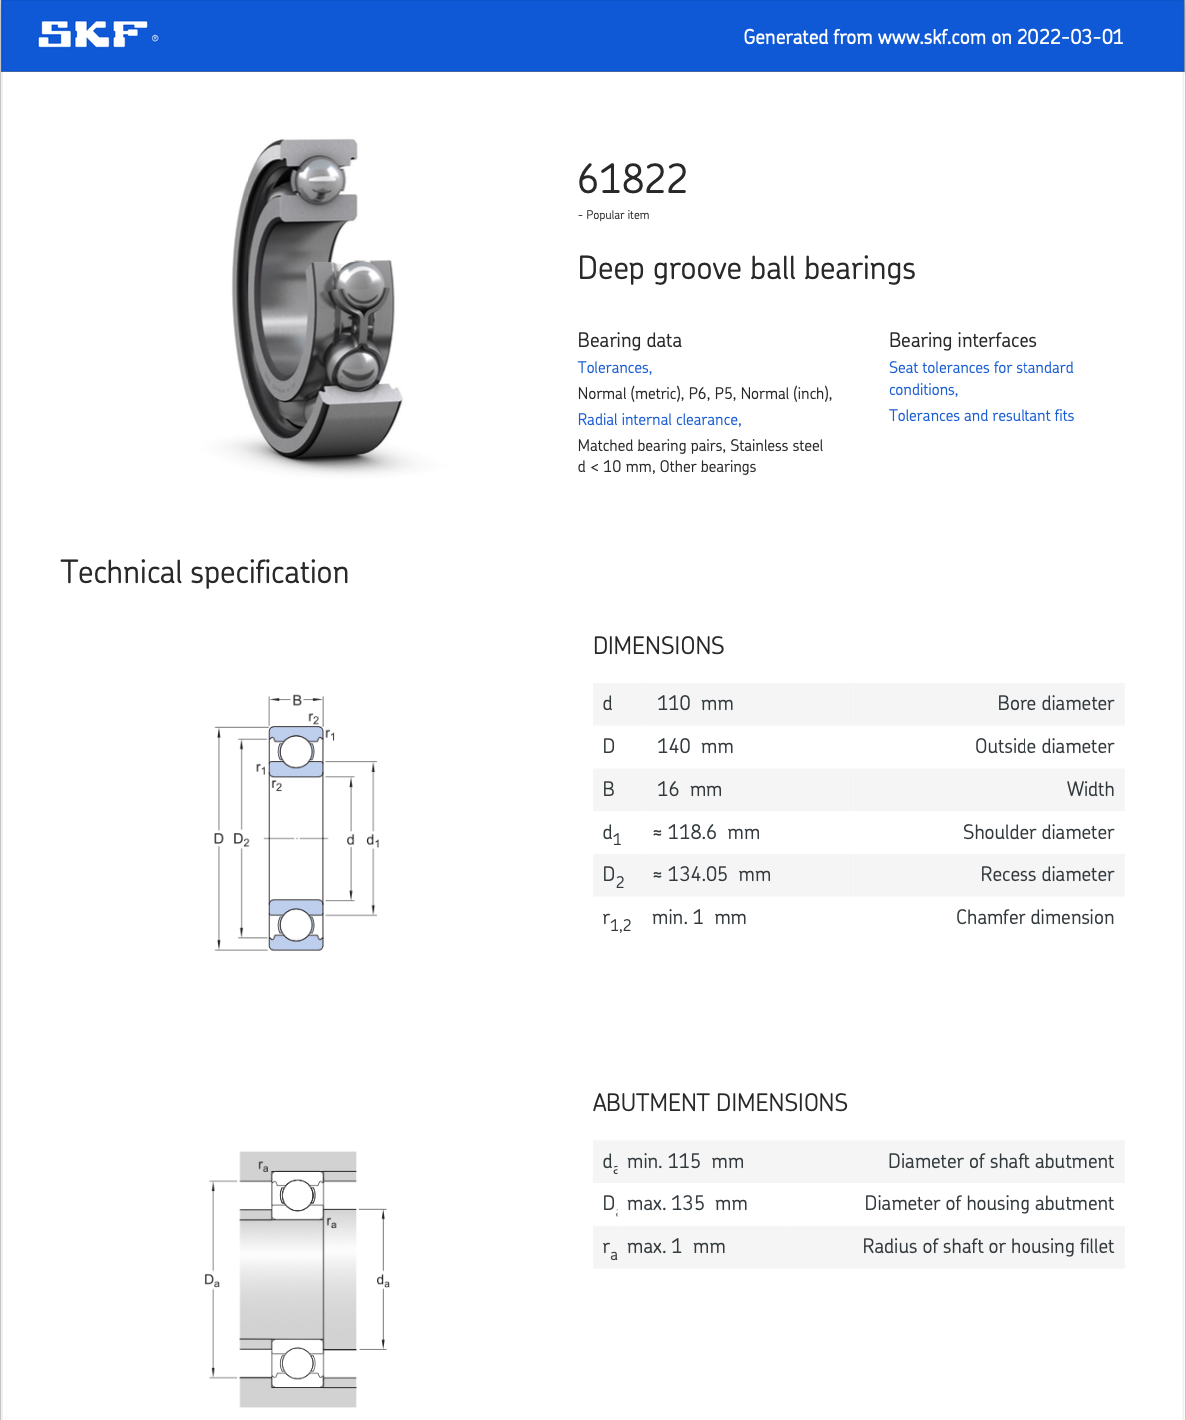
\includegraphics[scale=0.6]{Immagini/Cuscinetti3Albero5.png}
    \caption{Caratteristiche tecniche dei cuscinetti montati sull'albero 5}
    \label{fig:Cuscinetti3Albero5}
\end{figure}
\newpage
\begin{figure}[h]
    \centering
    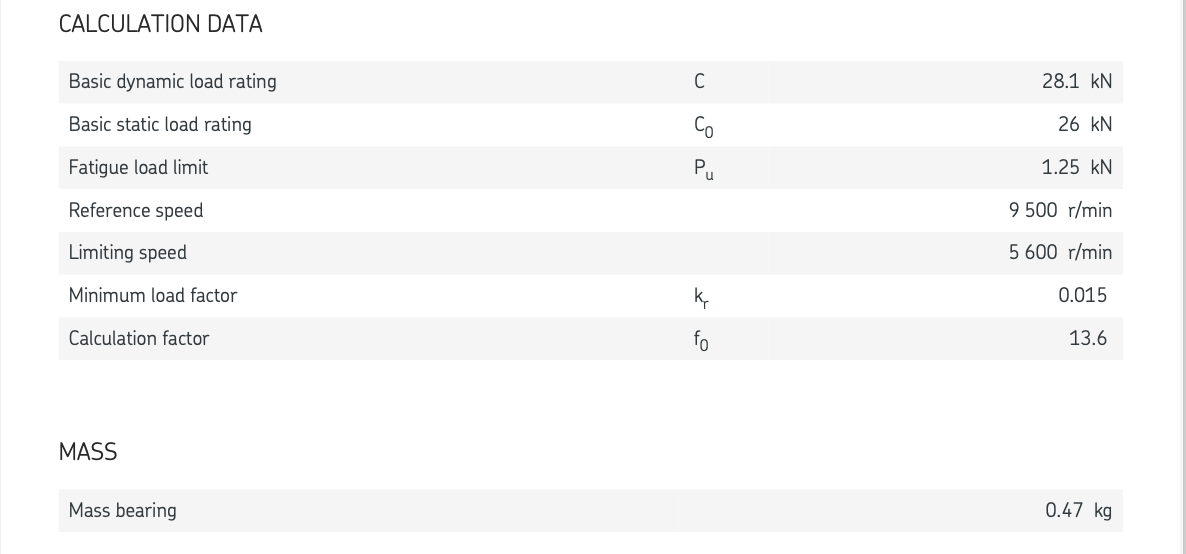
\includegraphics[scale=0.6]{Immagini/Cuscinetti4Albero5.png}
    \caption{Altre caratteristiche tecniche dei cuscinetti montati sull'albero 5}
        \label{fig:Cuscinetti4Albero5}
\end{figure}

Dalla progettazione degli alberi con il software KissSoft sono stati ottenuti i seguenti risultati per i cuscinetti.
\begin{figure}[h]
    \centering
    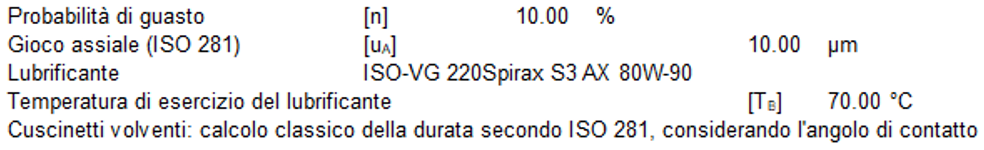
\includegraphics[scale=0.6]{Immagini/DettagliCuscinettiAlbero5.png}
    \caption{Alcuni dati notevoli riguardanti i cuscinetti dell'albero 5}
    \label{fig:DettagliCuscinettiAlbero5}
\end{figure}

Cuscinetto a rulli in basso.
\begin{figure}[h]
    \centering
        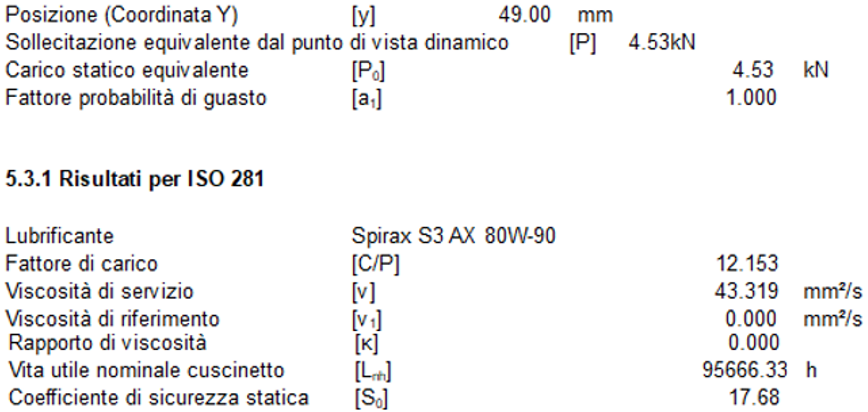
\includegraphics[scale=0.6]{Immagini/RisultatiCuscinettoBassoAlbero5.png}
    \caption{Risultati del cuscinetto in basso dell'albero 5}
    \label{fig:RisultatiCuscinettoBassoAlbero5}
\end{figure}
\newpage
Cuscinetto a sfere in alto.
\begin{figure}[h]
    \centering
    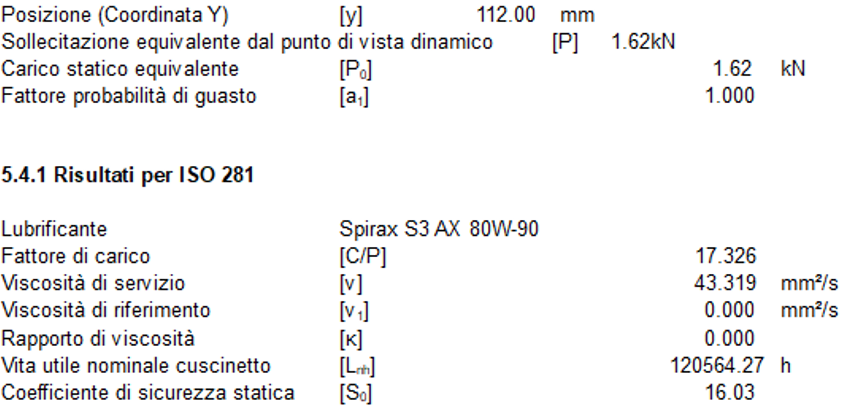
\includegraphics[scale=0.6]{Immagini/RisultatiCuscinettoAltoAlbero5.png}
    \caption{Risultati del cuscinetto in alto dell'albero 5}
    \label{fig:RisultatiCuscinettoAltoAlbero5}
\end{figure}

In conclusione.
\begin{figure}[h]
    \centering
    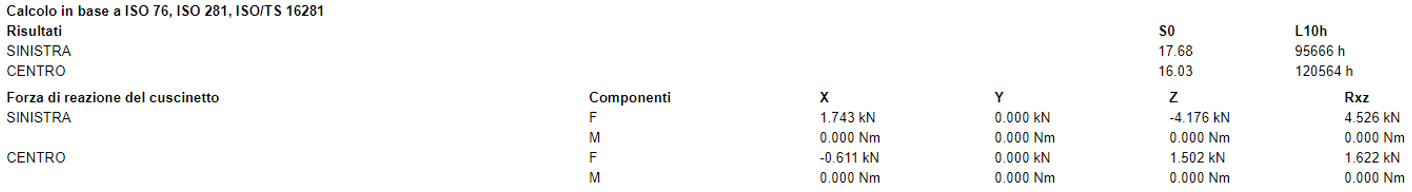
\includegraphics[scale=0.55]{Immagini/RisultatiCuscinettiAlbero5.png}
    \caption{Risultati complessivi dei cuscinetti per quanto riguarda l'albero 5}
    \label{fig:RisultatiCuscinettiAlbero5}
\end{figure}

Le caratteristiche geometriche dei singoli cuscinetti sono risultate funzionali alla realizzazione del modello tridimensionale del riduttore mediante SOLIDWORKS.\\
\\
Le informazioni dei cuscinetti montati sui diversi alberi sono state tutte ricavate dal catalogo SKF, dal quale poi sono stati anche scaricati i relativi modelli CAD già realizzati, pronti per la creazione del disegno di assieme.

